\documentclass[11pt]{article}

\usepackage{fullpage}
\usepackage{url}
\usepackage{mathtools}
\usepackage{graphicx}
\usepackage{listings}
\usepackage{color}

\definecolor{dkgreen}{rgb}{0,0.6,0}
\definecolor{gray}{rgb}{0.5,0.5,0.5}
\definecolor{mauve}{rgb}{0.58,0,0.82}

\lstset{frame=tb,
  aboveskip=3mm,
  belowskip=3mm,
  showstringspaces=false,
  columns=flexible,
  basicstyle={\small\ttfamily},
  numbers=none,
  numberstyle=\tiny\color{gray},
  keywordstyle=\color{blue},
  commentstyle=\color{dkgreen},
  stringstyle=\color{mauve},
  breaklines=true,
  breakatwhitespace=true,
  tabsize=3
}

\begin{document}
\thispagestyle{empty}
\parindent 0pt
\vfill
\large

\begin{center}
\LARGE{\bf \textsf{CS246: Mining Massive Data Sets}} \\*[4ex]
\end{center}

{\Large
\textbf{Assignment number:} 3
\vfill
\vfill

Fill in and include this cover sheet with each of your assignments. It is an honor code
violation to write down the wrong time. Assignments and code are due at 5:00 PM on Scoryst and SNAP respectively. Failure to include the coversheet with you assignment will
be penalized by 2 points.
Each student will have a total of \textit{two} free late periods. \textit{One late period expires at the start of
each class}. (Assignments are due on Thursdays, which means the first late period expires on
the following Tuesday at 5:00 PM.) Once these late periods are exhausted, any assignments
turned in late will be penalized 50\% per late period. However, no assignment will be accepted
more than one late period after its due date. (If an assignment is due to Thursday then we
will not accept it after the following Thursday.)
\vfill
\vfill
{\Large
\textbf{Your name:} \underline{Priyank Mathur} \\
\textbf{Email:} \underline{priyankm@stanford.edu} \textbf{SUNet ID:} \underline{priyankm}\\*[2ex] }
Collaborators: \underline{Emrah Budur, Shundan Xiao, Dibyajyoti Ghosh, Arkajyoti Misra} \\
\vfill

\vfill

I acknowledge and accept the Honor Code.\\*[3ex]
\bigskip
\textit{(Signed)} \underline{Priyank Mathur}
% If you are not printing this document out, just type your initials above

\vfill
\vfill

\pagebreak[4]
\section*{Answer to Question 1.a}

$$\epsilon_{iu} = 2 \times (R_{iu} - q_i . p_u^T)$$
$$q_i = q_i + \eta ( \epsilon_{iu} p_u - \lambda q_i)$$
$$p_u= p_u + \eta ( \epsilon_{iu} q_i - \lambda p_u)$$

Note that the factor 2 obtained during differentiation w.r.t $p_u$ and $q_i$ has been consumed within the learning rate $\eta$.

\pagebreak[4]
\section*{Answer to Question 1.b}

$\eta = 0.005$\\
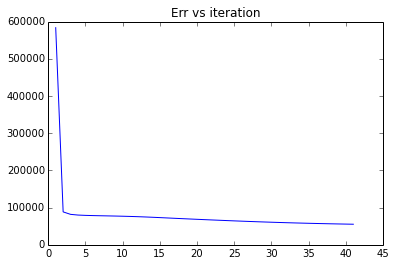
\includegraphics[scale=1]{q1errvsiter}


\pagebreak[4]
\section*{Answer to Question 1.c}
$Error_{tr}$ vs. k for $ \lambda = 0$\

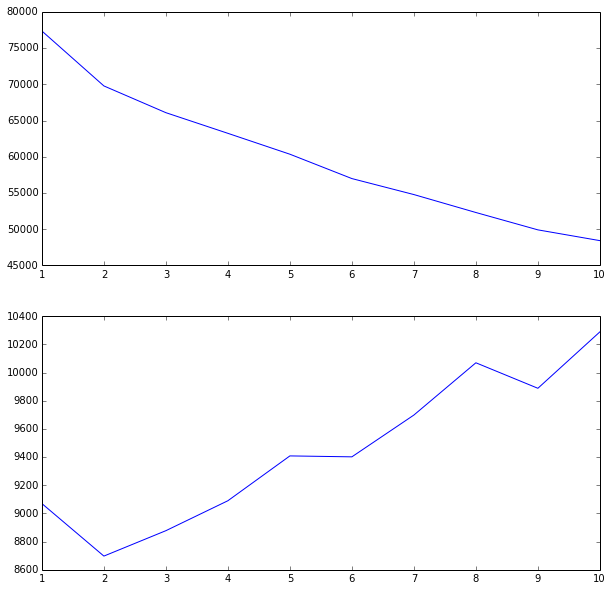
\includegraphics[scale=0.8]{q1errtrverrtel0}\

$Error_{te}$ vs. k for $ \lambda = 0$\
\\\\\\\\\

$Error_{tr}$ vs. k for $ \lambda = 0.2$\

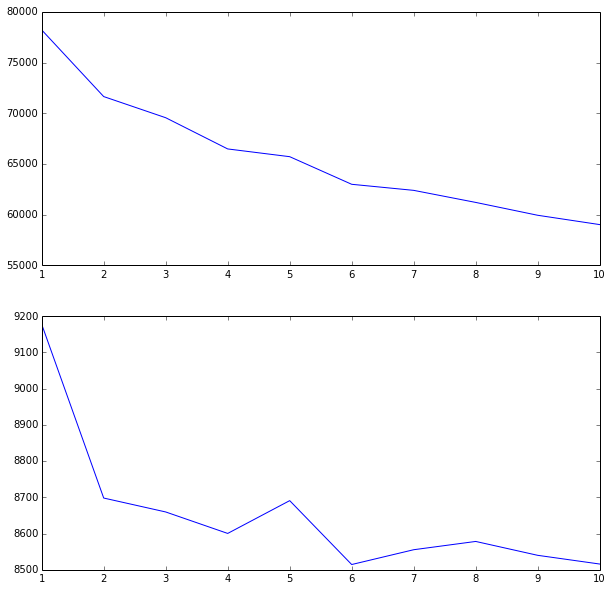
\includegraphics[scale=0.8]{q1errtrverrtel02}\

$Error_{te}$ vs. k for $ \lambda = 0.2$\\

Based on these graphs, we find the following to be true - 
\begin{itemize}
\item B: Regularization decreases the test error for $k \geq 5$
\item D: Regularization increases the training error for all (or almost all) k
\item H: Regularization decreases overfitting
\end{itemize}

\pagebreak[4]
\section*{Answer to Question 1.d}

$$\epsilon_{iu} = 2 \times (R_{iu} - (\mu + b_u + b_i + q_i . p_u^T))$$
$$q_i = q_i + \eta_{LF} ( \epsilon_{iu} p_u - \lambda q_i)$$
$$p_u= p_u + \eta_{LF} ( \epsilon_{iu} q_i - \lambda p_u)$$

$$b_{i_i} = b_{i_i} + \eta_{b_i} ( \epsilon_{iu} - \lambda b_{i_i})$$
$$b_{u_u} = b_{u_u} + \eta_{b_u} ( \epsilon_{iu} - \lambda b_{u_u})$$

$$\eta_{LF} = 0.005$$
$$\eta_{b_i} = 0.01$$
$$\eta_{b_u} = 0.01$$

\vspace{14cm}
$Error_{tr}$ vs. k for $ \lambda = 0$\

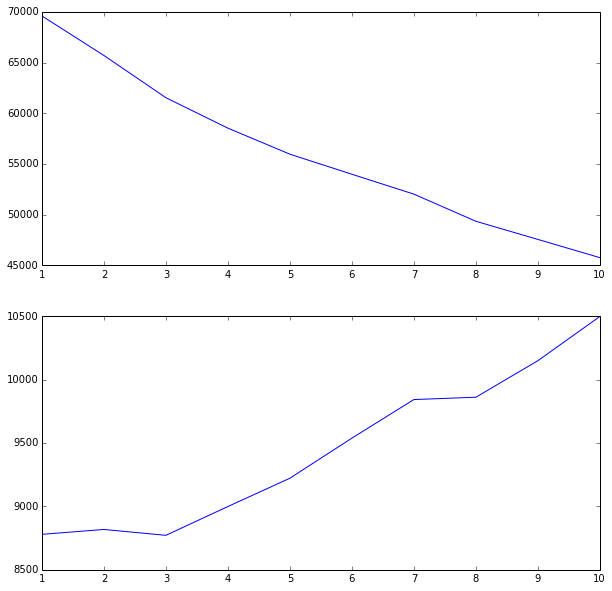
\includegraphics[scale=0.7]{q1errtrverrtelbias0}\

$Error_{te}$ vs. k for $ \lambda = 0$\

\vspace{8cm}
$Error_{tr}$ vs. k for $ \lambda = 0.2$\

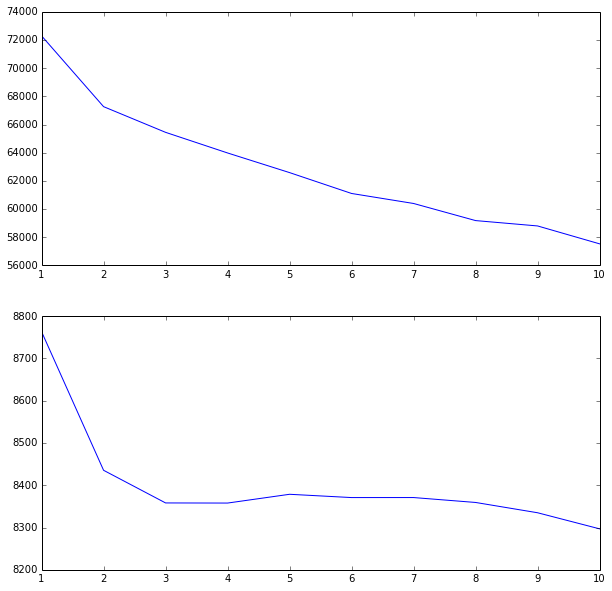
\includegraphics[scale=0.8]{q1errtrverrtelbias02}\

$Error_{te}$ vs. k for $ \lambda = 0.2$\\

Based on these graphs, we find the following to be true - 
\begin{itemize}
\item B: Regularization decreases the test error for $k \geq 5$
\item D: Regularization increases the training error for all (or almost all) k
\item H: Regularization decreases overfitting
\end{itemize}


\pagebreak[4]
\section*{Answer to Question 2a}



\pagebreak[4]
\section*{Answer to Question 2b}

\pagebreak[4]
\section*{Answer to Question 2c}

\pagebreak[4]
\section*{Answer to Question 2d}
Runtime for 40 iterations of power iteration - 791 $\mu s$.\\

Avg runtime for Monte Carlo with R = 1 - 7.83 $ms$.\

Avg runtime for Monte Carlo with R = 3 - 20.6 $ms$.\

Avg runtime for Monte Carlo with R = 5 - 35.57 $ms$.\\

\begin{tabular}{l | c | r}
\hline R & K & Error \\
\hline 1 & 10 & 0.0060365444268\\
\hline 1 & 30 & 0.0047717255253\\
\hline 1 & 50 & 0.0038620385493\\
\hline 1 & 100 & 0.0029277461094\\
\hline 3 & 10 & 0.0034659740412\\
\hline 3 & 30 & 0.0026577309646\\
\hline 3 & 50 & 0.0022720065398\\
\hline 3 & 100 & 0.0017132042790\\
\hline 5 & 10 & 0.0026678865383\\
\hline 5 & 30 & 0.0021502352960\\
\hline 5 & 50 & 0.0017972828358\\
\hline 5 & 100 & 0.0013425298758\\
\hline
\end{tabular}
\vspace{10mm}

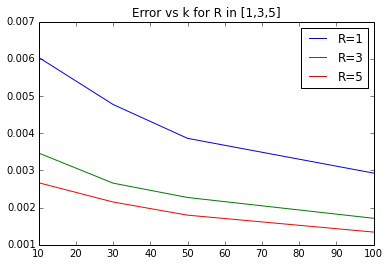
\includegraphics[scale=0.8]{q2d}\


\pagebreak[4]
\section*{Answer to Question 3.a}

$s_A(cameras, phones) = \dfrac{C1}{3 \times 2} [s_B(nokia.com,nokia.com) +  s_B(nokia.com,apple.com) \
 + s_B(kodak.com,nokia.com) + s_B(kodak.com,apple.com) + s_B(cannon.com,nokia.com) +\ s_B(cannon.com,apple.com)]$
 
$s_A(cameras, phones) =  \dfrac{0.8}{6} [1+0+0+0+0+0] = 0.13333$\

\vspace{0.5cm}
\begin{small}
\textbf{Iteration 1 -} \\
$s_A('cameras', 'cameras'): 1,\\
\mathbf {s_A('cameras', 'phones'): 0.13333333333333333},\\
s_A('printers', 'printers'): 1,\\
s_A('phones', 'phones'): 1,\\
\mathbf {s_A('cameras', 'printers'): 0.0},\\
s_A('phones', 'printers'): 0.0\\
\\
s_B('cannon.com', 'nokia.com'): 0.4, \\
s_B('hp.com', 'nokia.com'): 0.0, \\
s_B('kodak.com', 'kodak.com'): 1, \\
s_B('apple.com', 'kodak.com'): 0.0, \\
s_B('cannon.com', 'kodak.com'): 0.8, \\
s_B('cannon.com', 'cannon.com'): 1, \\
s_B('hp.com', 'kodak.com'): 0.0, \\
s_B('apple.com', 'hp.com'): 0.0, \\
s_B('kodak.com', 'nokia.com'): 0.4, \\
s_B('apple.com', 'apple.com'): 1, \\
s_B('apple.com', 'nokia.com'): 0.4, \\
s_B('nokia.com', 'nokia.com'): 1, \\
s_B('cannon.com', 'hp.com'): 0.0, \\
s_B('hp.com', 'hp.com'): 1, \\
s_B('apple.com', 'cannon.com'): 0.0$

\vspace{0.5cm}
\textbf{Iteration 2 -} \\
$s_A('cameras', 'cameras'): 1, \\
\mathbf {s_A('cameras', 'phones'): 0.2933333333333333}, \\
s_A('printers', 'printers'): 1, \\
s_A('phones', 'phones'): 1, \\
\mathbf {s_A('cameras', 'printers'): 0.0}, \\
s_A('phones', 'printers'): 0.0\\
\\
s_B('cannon.com', 'nokia.com'): 0.45333333333333337, \\
s_B('hp.com', 'nokia.com'): 0.0, \\
s_B('kodak.com', 'kodak.com'): 1, \\
s_B('apple.com', 'kodak.com'): 0.10666666666666667, \\
s_B('cannon.com', 'kodak.com'): 0.8, \\
s_B('cannon.com', 'cannon.com'): 1, \\
s_B('hp.com', 'kodak.com'): 0.0, \\
s_B('apple.com', 'hp.com'): 0.0, \\
s_B('kodak.com', 'nokia.com'): 0.45333333333333337, \\
s_B('apple.com', 'apple.com'): 1, \\
s_B('apple.com', 'nokia.com'): 0.45333333333333337, \\
s_B('nokia.com', 'nokia.com'): 1, \\
s_B('cannon.com', 'hp.com'): 0.0, \\
s_B('hp.com', 'hp.com'): 1, \\
s_B('apple.com', 'cannon.com'): 0.10666666666666667$

\vspace{0.5cm}
\textbf{Iteration 3 -} \\
$s_A('cameras', 'cameras'): 1, \\
\mathbf {s_A('cameras', 'phones'): 0.34311111111111114}, \\
s_A('printers', 'printers'): 1, \\
s_A('phones', 'phones'): 1, \\
\mathbf {s_A('cameras', 'printers'): 0.0}, \\
s_A('phones', 'printers'): 0.0\\
\\
s_B('cannon.com', 'nokia.com'): 0.5173333333333333, \\
s_B('hp.com', 'nokia.com'): 0.0, \\
s_B('kodak.com', 'kodak.com'): 1, \\
s_B('apple.com', 'kodak.com'): 0.23466666666666663, \\
s_B('cannon.com', 'kodak.com'): 0.8, \\
s_B('cannon.com', 'cannon.com'): 1, \\
s_B('hp.com', 'kodak.com'): 0.0, \\
s_B('apple.com', 'hp.com'): 0.0, \\
s_B('kodak.com', 'nokia.com'): 0.5173333333333333, \\
s_B('apple.com', 'apple.com'): 1, \\
s_B('apple.com', 'nokia.com'): 0.5173333333333333, \\
s_B('nokia.com', 'nokia.com'): 1, \\
s_B('cannon.com', 'hp.com'): 0.0, \\
s_B('hp.com', 'hp.com'): 1, \\
s_B('apple.com', 'cannon.com'): 0.23466666666666663$
\end{small}\\

Final result after 3 iterations - \\
$
\mathbf {s_A('cameras', 'phones'): 0.34311111111111114}, \\
\mathbf {s_A('cameras', 'printers'): 0.0} \\
$

\pagebreak[4]
\section*{Answer to Question 3.b}

\setcounter{equation}{2}

\begin{small}
\begin{equation}
s_A (X, Y) = \dfrac{C1}{\sum_{i=1}^{|O(X)|} \sum_{j=1}^{|O(Y)|} W_{X, O_i(X)} \cdot W_{Y, O_j(Y)}} \times
\sum_{i=1}^{|O(X)|} \sum_{j=1}^{|O(Y)|} W_{X, O_i(X)} \cdot W_{Y, O_j(Y)} \cdot s_B(O_i(X), O_j (Y ))
\end{equation}
\end{small}

\begin{small}
\begin{equation}
s_B (x, y) = \dfrac{C2}{\sum_{i=1}^{|I(x)|} \sum_{j=1}^{|I(y)|} \cdot W_{I_i(x), x} W_{I_j(y), y}} \times
\sum_{i=1}^{|I(x)|} \sum_{j=1}^{|I(y)|} W_{I_i(x), x} \cdot W_{I_j(y), y} \cdot s_A(I_i(x), I_j (y ))
\end{equation}
\end{small}


\pagebreak[4]
\section*{Answer to Question 3.c}


\pagebreak[4]
\section*{Answer to Question 4a}


\pagebreak[4]
\section*{Answer to Question 4b}

\pagebreak[4]
\section*{Answer to Question 4c}


\subsection*{1}
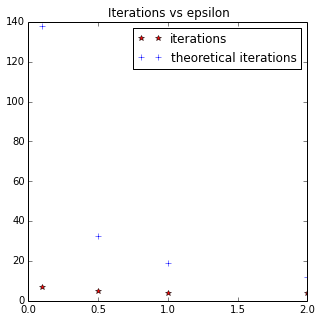
\includegraphics[scale=0.8]{q4c1}\\

\vspace{2cm}

\begin{tabular}{l | c | r}
\hline $\epsilon$ & Iterations & Theoretical iterations \\
\hline 0.1 & 7 & 137.67\\
\hline 0.5 & 5 & 32.36\\
\hline 1 & 4 & 18.93\\
\hline 2 & 3 & 11.94\\
\hline
\end{tabular}

\pagebreak[4]
\subsection*{2}
\

Density $(\rho(S_i))$ vs iteration\\
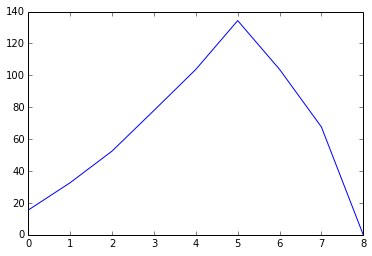
\includegraphics[scale=0.8]{q4c2density}\
\vspace{3cm}

$|E(S_i)|$ vs iteration\\
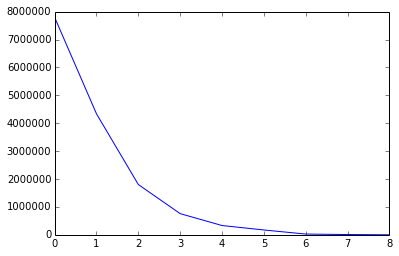
\includegraphics[scale=0.8]{q4c2indsetcnt}\\
\vspace{3cm}

$|S_i|$ vs iteration\\
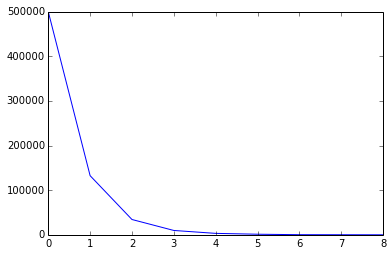
\includegraphics[scale=0.8]{q4c2scnt}\


\pagebreak[4]
\subsection*{3}
\

Density $(\rho(\bar{S_j}))$ vs iteration\\
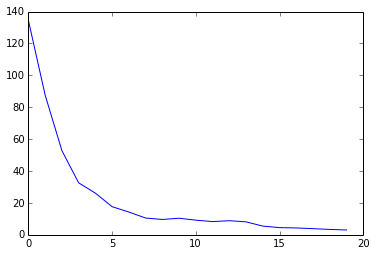
\includegraphics[scale=0.8]{q4c3densitycnt}\
\vspace{3cm}

$|E(\bar{S_j})|$ vs iteration\\
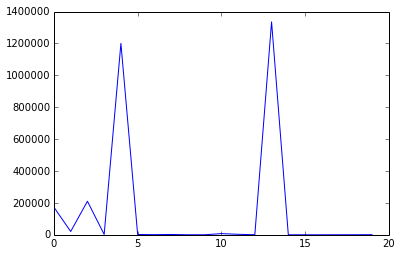
\includegraphics[scale=0.8]{q4c3essacnt}\\
\vspace{3cm}

$|\bar{S_j}|$ vs iteration\\
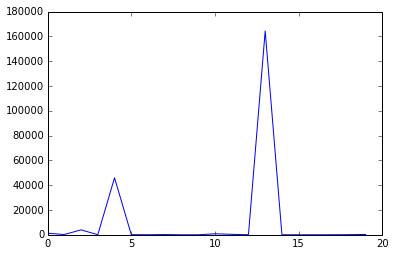
\includegraphics[scale=0.8]{q4c3scnt}\


\pagebreak[4]
\section*{Code for Q1}

\iffalse
\lstinputlisting[language=Python]{submission/snap/priyankm_hw2_q1.txt}
\fi

\pagebreak[4]
\section*{Code for Q2}

\pagebreak[4]
\section*{Code for Q4}


\end{document}
